\subtitlesection{Ring of Mind Shielding}
{Ring, uncommon (requires attunement)}
\noindent{While wearing this ring, you are immune to magic that allows other creatures to read your thoughts, determine whether you are lying, know your alignment, or know your creature type. Creatures can telepathically communicate with you only if you allow it.}

You can use an action to cause the ring to become invisible until you use another action to make it visible, until you remove the ring, or until you die.

If you die while wearing the ring, your soul enters it, unless it already houses a soul. You can remain in the ring or depart for the afterlife. As long as your soul is in the ring, you can telepathically communicate with any creature wearing it. A wearer can't prevent this telepathic communication.

\subtitlesection{“I Can’t Believe It’s Not Necromancy!”}
{Wand, uncommon}
\noindent{This wand has 3 charges. While holding it, you can use an action to expend one of its charges to cast the \textit{cure wounds} spell from it. The wand regains its expended charges daily at dawn.}

\begin{figure}[h]
	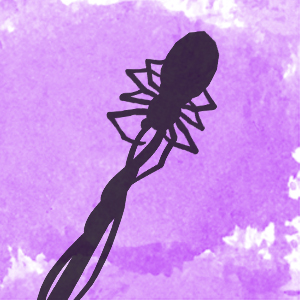
\includegraphics[width=\columnwidth-\columnsep]{wand}
\end{figure}
% {\vspace{-3em}}
